%----------
%   IMPORTANTE
%----------

% Si nunca has utilizado LaTeX es conveniente que aprendas una serie de conceptos básicos antes de utilizar esta plantilla. Te aconsejamos que leas previamente algún tutorial (puedes encontar muchos en Internet).

% Esta plantilla está basada en las recomendaciones de la guía "Trabajo fin de Grado: Escribir el TFG", que encontrarás en http://uc3m.libguides.com/TFG/escribir
% contiene recomendaciones de la Biblioteca basadas principalmente en estilos APA e IEEE, pero debes seguir siempre las orientaciones de tu Tutor de TFG y la normativa de TFG para tu titulación.

% Encontrarás un ejemplo de TFG realizado con esta misma plantilla en la carpeta "_ejemplo_TFG_2019". Consúltalo porque contiene ejemplos útiles para incorporar tablas, figuras, listados de código, bibliografía, etc.


%----------
%	CONFIGURACIÓN DEL DOCUMENTO
%----------

% Definimos las características del documento y añadimos una serie de paquetes (\usepackage{package}) que agregan funcionalidades a LaTeX.

\documentclass[12pt]{report} %fuente a 12pt


\usepackage{lipsum} % el paquete lipsum permite rellenar texto del tipo "Lorem ipsum" a modo de ejemplo

% MÁRGENES: 2,5 cm sup. e inf.; 3 cm izdo. y dcho.
\usepackage[
a4paper,
vmargin=2.5cm,
hmargin=3cm
]{geometry}


% INTERLINEADO: Estrecho (6 ptos./interlineado 1,15) o Moderado (6 ptos./interlineado 1,5)
\renewcommand{\baselinestretch}{1.15}
\parskip=6pt

% DEFINICIÓN DE COLORES para portada y listados de código
 
\usepackage[table , svgnames]{xcolor}
\usepackage{listings}

\lstset{language=R,
    basicstyle=\small\ttfamily,
    stringstyle=\color{DarkGreen},
    otherkeywords={0,1,2,3,4,5,6,7,8,9},
    morekeywords={TRUE,FALSE},
    deletekeywords={data,frame,length,as,character},
    keywordstyle=\color{blue},
    commentstyle=\color{DarkGreen},
}

\definecolor{azulUC3M}{RGB}{0,0,102}
\definecolor{gray97}{gray}{.97}
\definecolor{gray75}{gray}{.75}
\definecolor{gray45}{gray}{.45}

% Soporte para GENERAR PDF/A --es importante de cara a su inclusión en e-Archivo porque es el formato óptimo de preservación y a la generación de metadatos, tal y como se describe en http://uc3m.libguides.com/ld.php?content_id=31389625. En la carpeta incluímos el archivo plantilla_tfg_2017.xmpdata en el que puedes incluir los metadatos que se incorporarán al archivo PDF cuando lo compiles. Ese archivo debe llamarse igual que tu archivo .tex. Puedes ver un ejemplo en esta misma carpeta.
\usepackage[a-1b]{pdfx}

% ENLACES
\usepackage{hyperref}
\hypersetup{colorlinks=true,
	linkcolor=black, % enlaces a partes del documento (p.e. índice) en color negro
	urlcolor=blue} % enlaces a recursos fuera del documento en azul

% EXPRESIONES MATEMATICAS
\usepackage{amsmath,amssymb,amsfonts,amsthm}

\usepackage{txfonts} 
\usepackage[T1]{fontenc}
\usepackage[utf8]{inputenc}

\usepackage[spanish, es-tabla]{babel} % información sobre el paquete babel para español http://osl.ugr.es/CTAN/language/spanish/babel/base/spanish.pdf
\usepackage[babel, spanish=spanish]{csquotes}
\AtBeginEnvironment{quote}{\small}

% diseño de PIE DE PÁGINA
\usepackage{fancyhdr}
\pagestyle{fancy}
\fancyhf{}
\renewcommand{\headrulewidth}{0pt}
\rfoot{\thepage}
\fancypagestyle{plain}{\pagestyle{fancy}}

% DISEÑO DE LOS TÍTULOS de las partes del trabajo (capítulos y epígrafes o subcapítulos)
\usepackage{titlesec}
\usepackage{titletoc}
\titleformat{\chapter}[block]
{\large\bfseries\filcenter}
{\thechapter.}
{5pt}
{\MakeUppercase}
{}
\titlespacing{\chapter}{0pt}{0pt}{*3}
\titlecontents{chapter}
[0pt]                                               
{}
{\contentsmargin{0pt}\thecontentslabel.\enspace\uppercase}
{\contentsmargin{0pt}\uppercase}                        
{\titlerule*[.7pc]{.}\contentspage}                 

\titleformat{\section}
{\bfseries}
{\thesection.}
{5pt}
{}
\titlecontents{section}
[5pt]                                               
{}
{\contentsmargin{0pt}\thecontentslabel.\enspace}
{\contentsmargin{0pt}}
{\titlerule*[.7pc]{.}\contentspage}

\titleformat{\subsection}
{\normalsize\bfseries}
{\thesubsection.}
{5pt}
{}
\titlecontents{subsection}
[10pt]                                               
{}
{\contentsmargin{0pt}                          
	\thecontentslabel.\enspace}
{\contentsmargin{0pt}}                        
{\titlerule*[.7pc]{.}\contentspage}  

%%%%%%%%%%%%%%%%
\usepackage{tcolorbox}
\tcbuselibrary{listingsutf8}
\tcbuselibrary{theorems}
\usepackage[short]{optidef}
 \usepackage[short]{optidef}
\usepackage{listings}
\usepackage{multirow}

% DISEÑO DE TABLAS. Puedes elegir entre el estilo para ingeniería o para ciencias sociales y humanidades. Por defecto, está activado el estilo de ingeniería. Si deseas utilizar el otro, comenta las líneas del diseño de ingeniería y descomenta las del diseño de ciencias sociales y humanidades
\usepackage{multirow} % permite combinar celdas 
\usepackage{caption} % para personalizar el título de tablas y figuras
\usepackage{floatrow} % utilizamos este paquete y sus macros \ttabbox y \ffigbox para alinear los nombres de tablas y figuras de acuerdo con el estilo definido. Para su uso ver archivo de ejemplo 
\usepackage{array} % con este paquete podemos definir en la siguiente línea un nuevo tipo de columna para tablas: ancho personalizado y contenido centrado
\newcolumntype{P}[1]{>{\centering\arraybackslash}p{#1}}
\DeclareCaptionFormat{upper}{#1#2\uppercase{#3}\par}

% Diseño de tabla para ingeniería
\captionsetup[table]{
	format=upper,
	name=TABLA,
	justification=centering,
	labelsep=period,
	width=.75\linewidth,
	labelfont=small,
	font=small,
}

%Diseño de tabla para ciencias sociales y humanidades
%\captionsetup[table]{
%	justification=raggedright,
%	labelsep=period,
%	labelfont=small,
%	singlelinecheck=false,
%	font={small,bf}
%}

% DISEÑO DE FIGURAS. Puedes elegir entre el estilo para ingeniería o para ciencias sociales y humanidades. Por defecto, está activado el estilo de ingeniería. Si deseas utilizar el otro, comenta las líneas del diseño de ingeniería y descomenta las del diseño de ciencias sociales y humanidades
\usepackage{graphicx}
\graphicspath{{imagenes/}} %ruta a la carpeta de imágenes

% Diseño de figuras para ingeniería
\captionsetup[figure]{
	format=hang,
	name=Fig.,
	singlelinecheck=off,
	labelsep=period,
	labelfont=small,
	font=small		
}

% Diseño de figuras para ciencias sociales y humanidades
%\captionsetup[figure]{
%	format=hang,
%	name=Figura,
%	singlelinecheck=off,
%	labelsep=period,
%	labelfont=small,
%	font=small		
%}


% NOTAS A PIE DE PÁGINA
\usepackage{chngcntr} %para numeración contínua de las notas al pie
\counterwithout{footnote}{chapter}

% LISTADOS DE CÓDIGO
% soporte y estilo para listados de código. Más información en https://es.wikibooks.org/wiki/Manual_de_LaTeX/Listados_de_código/Listados_con_listings
\usepackage{listings}

% definimos un estilo de listings
\lstdefinestyle{estilo}{ frame=Ltb,
	framerule=0pt,
	aboveskip=0.5cm,
	framextopmargin=3pt,
	framexbottommargin=3pt,
	framexleftmargin=0.4cm,
	framesep=0pt,
	rulesep=.4pt,
	backgroundcolor=\color{gray97},
	rulesepcolor=\color{black},
	%
	basicstyle=\ttfamily\footnotesize,
	keywordstyle=\bfseries,
	stringstyle=\ttfamily,
	showstringspaces = false,
	commentstyle=\color{gray45},     
	%
	numbers=left,
	numbersep=15pt,
	numberstyle=\tiny,
	numberfirstline = false,
	breaklines=true,
	xleftmargin=\parindent
}

\captionsetup[lstlisting]{font=small, labelsep=period}
% fijamos el estilo a utilizar 
\lstset{style=estilo}
\renewcommand{\lstlistingname}{\uppercase{Código}}


%BIBLIOGRAFÍA - PUEDES ELEGIR ENTRE ESTILO IEEE O APA. POR DEFECTO ESTÁ CONFIGURADO IEEE. SI DESEAS USAR APA, COMENTA LAS LÍNEA DE IEEE Y DESCOMENTA LAS DE APA. Si haces cambios en la configuración de la bibliografía y no obtienes los resultados esperados, es recomendable limpiar los archivos auxiliares y volver a compilar en este orden: COMPILAR-BIBLIOGRAFIA-COMPILAR

% Tienes más información sobre cómo generar bibliografía y CONFIGURAR TU EDITOR DE TEXTO para compilar con biber en http://tex.stackexchange.com/questions/154751/biblatex-with-biber-configuring-my-editor-to-avoid-undefined-citations , https://www.overleaf.com/learn/latex/Bibliography_management_in_LaTeX y en http://www.ctan.org/tex-archive/macros/latex/exptl/biblatex-contrib
% También te recomendamos consultar la guía temática de la Biblioteca sobre citas bibliográficas: http://uc3m.libguides.com/guias_tematicas/citas_bibliograficas/inicio

% CONFIGURACIÓN PARA LA BIBLIOGRAFÍA IEEE
\usepackage[backend=biber, style=ieee, isbn=false,sortcites, maxbibnames=5, minbibnames=1]{biblatex} % Configuración para el estilo de citas de IEEE, recomendado para el área de ingeniería. "maxbibnames" indica que a partir de 5 autores trunque la lista en el primero (minbibnames) y añada "et al." tal y como se utiliza en el estilo IEEE.

%CONFIGURACIÓN PARA LA BIBLIOGRAFÍA APA
%\usepackage[style=apa, backend=biber, natbib=true, hyperref=true, uniquelist=false, sortcites]{biblatex}
%\DeclareLanguageMapping{spanish}{spanish-apa}

% Añadimos las siguientes indicaciones para mejorar la adaptación de los estilos en español
\DefineBibliographyStrings{spanish}{%
	andothers = {et\addabbrvspace al\adddot}
}
\DefineBibliographyStrings{spanish}{
	url = {\adddot\space[En línea]\adddot\space Disponible en:}
}
\DefineBibliographyStrings{spanish}{
	urlseen = {Acceso:}
}
\DefineBibliographyStrings{spanish}{
	pages = {pp\adddot},
	page = {p.\adddot}
}

\addbibresource{bibliografia/bibliografia.bib} % llama al archivo bibliografia.bib en el que debería estar la bibliografía utilizada






%-------------
%	DOCUMENTO
%-------------

\begin{document}

	\pagenumbering{roman}
	
	%----------
	%	PORTADA
	%----------	
	\begin{titlepage}
		\begin{sffamily}
			\color{azulUC3M}
			\begin{center}
				\begin{figure}[H] %incluimos el logotipo de la Universidad
					\makebox[\textwidth][c]{\includegraphics[width=16cm]{Portada_Logo.png}}
		%----------
				\end{figure}
			\vspace{2.5cm}
				\begin{Large}
					Grado Estadística y Empresa\\			
					2021/22\\
					\vspace{1cm}		
				%	\textsl{}
					\bigskip
		%---------------
					
				\end{Large}
				{\Huge Distancias Estadisticas: \\ \vspace*{0.3cm}
				
				Teoria y Aplicaciones }\\
				\vspace*{0.5cm}
				\rule{10.5cm}{0.1mm}\\
				\vspace*{0.9cm}
				{\LARGE Fabio Scielzo Ortiz}\\ 
				\vspace*{1cm}
				\begin{Large}
					%Tutor/es\\
					%nombre\\
					%Lugar y fecha de presentación prevista\\
				\end{Large}
			\end{center}
			\vfill
			\color{black}
			
			% si nuestro trabajo se va a publicar con una licencia Creative Commons, incluir estas líneas. Es la opción recomendada.
			%\includegraphics[width=4.2cm]{imagenes/creativecommons.png}\\ %incluimos el logotipo de creativecommons
			%\emph{[Incluir en el caso del interés en su publicación en el archivo abierto]}\\  % BORRAR ESTA LÍNEA
			%Esta obra se encuentra sujeta a la licencia %Creative Commons \textbf{Reconocimiento - No Comercial - Sin Obra Derivada}
		\end{sffamily}
	\end{titlepage}
	
	\newpage %página en blanco o de cortesía
	\thispagestyle{empty}
	\mbox{}


%----------
%	ÍNDICES
%----------	

%--
%Índice general
%-
\tableofcontents
\thispagestyle{fancy}

\newpage %página en blanco o de cortesía
\thispagestyle{empty}
\mbox{}


%----------
%	TRABAJO
%----------	
\clearpage
\pagenumbering{arabic} % numeración con múmeros arábigos para el resto de la publicación	



\lstset{language=R,
    basicstyle=\small\ttfamily,
    stringstyle=\color{DarkGreen},
    otherkeywords={0,1,2,3,4,5,6,7,8,9},
    morekeywords={TRUE,FALSE},
    deletekeywords={data,frame,length,as,character},
    keywordstyle=\color{blue},
    commentstyle=\color{DarkGreen},
}


\chapter{Distancias Estadisticas:}

El concepto de distancia entre elementos de un conjunto $\varepsilon$ permite interpretar geometricamente muchas técnicas clásicas del análisis multivariante .

Esta interpretación es posible tanto con variables cuantitativas como categoricas, o incluso cuando no se dispone de variables, siempre que tenga sentido obtener una medida de proximidad entre los elementos de $\varepsilon$

\section{Definición de distancia:}

Dado un conjunto de elementos $\varepsilon$

\tcbset{colback=white!1!white,colframe=brown!78!black}
\begin{tcolorbox}[toptitle=2mm,title= Casi-Métrica:   ]
Se denomina \textbf{casi-metrica} o disimilaridad a toda aplicación $\delta : \varepsilon x \varepsilon \rightarrow \mathbb{R}$ que cumpla las siguientes propiedades:

1)\hspace{0.2cm} $\delta (i,j) \geq 0 \hspace{0.15cm}, \forall i,j $

2)\hspace{0.2cm} $\delta (i,i) = 0 \hspace{0.15cm}, \forall i $

3)\hspace{0.2cm} $\delta (i,j) = \delta (j, i) \hspace{0.15cm}, \forall i,j $

\end{tcolorbox}


\tcbset{colback=white!1!white,colframe=brown!78!black}
\begin{tcolorbox}[toptitle=2mm,title= Semi-Métrica:   ]
Se denomica \textbf{semi-metrica} a toda disimilaridad  que cumpla la desigualdad triangular:

4)\hspace{0.2cm} $\delta (i,j) \hspace{0.1 cm}\leq \hspace{0.1 cm} \delta (i,k) + \delta (k,i) \hspace{0.15cm}, \forall i,j,k$

\end{tcolorbox}

\tcbset{colback=white!1!white,colframe=brown!78!black}
\begin{tcolorbox}[toptitle=2mm,title= Métrica:   ]
Se denomina \textbf{metrica} a toda semi-metrica que cumple:

5)\hspace{0.2cm} $\delta (i,j)=0 \Leftrightarrow i=j$
\end{tcolorbox}

\tcbset{colback=white!1!white,colframe=brown!78!black}
\begin{tcolorbox}[toptitle=2mm,title= Distancia:   ]
Una \textbf{distancia} es una \textbf{métrica} o una \textbf{semi-métrica}
 \end{tcolorbox}
 
\newpage

\section{Matriz de distancias:}

Cuando $\varepsilon$ sea un conjunto finito , tendremos una matriz de distancias:
\tcbset{colback=white!1!white,colframe=brown!78!black}
\begin{tcolorbox}[toptitle=2mm,title= Matriz de distancias:   ]
\begin{gather*}
D= \begin{pmatrix}
0 & \delta_{12}&...&\delta_{1n}\\
\delta_{21} & 0&...&\delta_{2n}\\
...&...&...&...\\
\delta_{n1}& \delta_{n2}&...& 0\\
\end{pmatrix}
\end{gather*}

con $\delta_{ij}=\delta_{ji}$

\end{tcolorbox}

También usaremos la matriz de cuadrados de distancias:

\tcbset{colback=white!1!white,colframe=brown!78!black}
\begin{tcolorbox}[toptitle=2mm,title= Matriz de distancias al cuadrado:   ]
\begin{gather*}
D^{(2)}= \begin{pmatrix}
0 & \delta^2_{12}&...&\delta^2_{1n}\\
\delta^2_{21} & 0&...&\delta^2_{2n}\\
...&...&...&...\\
\delta^2_{n1}& \delta^2_{n2}&...& 0\\
\end{pmatrix}
\end{gather*}

\end{tcolorbox}


No debe confundirse con  $D^2=D\cdot D$



\chapter{Distancias con variables cuantitativas:}

Sean $X_1,...,X_p$ variables cuantitativas, 

Sean $x_i=(x_{i1},...,x_{ip})^t$ \hspace{0.2cm}y\hspace{0.2cm}
$x_j=(x_{i1},...,x_{ip})^t$ los valores (observaciones) de las variables $X_1,...,X_p$ para los elementos o individuos $i$ y $j$ de la muestra.


\section{Distancia Euclidea:}

\tcbset{colback=white!1!white,colframe=brown!78!black}
\begin{tcolorbox}[toptitle=2mm,title= Distancia Euclidea:   ]
La distancia euclidea entre los elementos / individuos $i$ y $j$ respecto de las variables cuantitativas $X_1,...,X_p$ se define como:

\begin{gather*}
\delta^2(i,j)_{Euclidea} = \sum_{k=1}^{p} (x_{ik} - x_{jk})\hspace{0.05cm}^2 = (x_i - x_j)\hspace{0.05cm}^t\cdot (x_i - x_j) \\ \\
\delta(i,j)_{Euclidea} =\sqrt{\sum_{k=1}^{p} (x_{ik} - x_{jk})\hspace{0.05cm}^2  }  = \sqrt{(x_i - x_j)\hspace{0.05cm}^t\cdot (x_i - x_j)}
\end{gather*}

\end{tcolorbox}

\vspace{0.2cm}

\subsection{Inconvenientes:}

Pese a que es una de las distancias mas conocidas no es adecuada en muchos casos por las siguientes razones:

1) \hspace{0.15cm} \textbf{Presupone} que las \textbf{variables} son \textbf{incorreladas} y con \textbf{varianza unidad} (aunque este problema puede solventarse estandarizando las variables a varianza unidad dividiendolas entre sus respectivas desviaciones tipicas). 

2) \hspace{0.15cm} \textbf{No} es \textbf{invariante frente a cambios de escala} (cambios de unidades de medida) de las variables.

\vspace{0.6cm}

Veamos que significa esto ultimo con mas detalle:

Si se aplica un cambio de escala a las variables $a\cdot X_j + b$, con $a\neq 1$ y $b\neq 0$

Ahora las observaciones para los elementos $i$ y $j$ son $a\cdot x_i + b$ y $a\cdot x_j + b$ 

Entonces la distancia euclidea entre los elementos $i$ y $j$ respecto de las variables escaladas $a\cdot X_j + b$ es:

\begin{gather*}
\delta^2(i,j)_{Euclidea} = a^2 \cdot (x_i - x_j)^t\cdot (x_i - x_j)
\end{gather*}


\subsection{Aplicación en R: Data-set}

Data-set de trabajo, tendra 4 variables cuantitativas, 3 binarias y 3 categoricas multiples:

\begin{lstlisting}
#Cuantitativas
X1 <- rnorm(50, mean=10 , sd=15)
X2 <- rnorm(50, mean=10 , sd=15)
X3 <- rnorm(50, mean=10 , sd=15)
X4 <- rnorm(50, mean=10 , sd=15)

#Binarias 
X5<- round(runif(50))
X6<- round(runif(50))
X7<- round(runif(50))

#Categoricas multiples 
X8<-round(runif(50, min=0, max=4)) #categorias: 0,1,2,3,4
X9<-round(runif(50, min=0, max=3))  #categorias: 0,1,2,3
X10<-round(runif(50, min=0, max=5))  #categorias: 0,1,2,3,4,5
\end{lstlisting}

 
\begin{lstlisting}
library(tidyverse)
 
Datos_Mixtos<-tibble(X1,X2,X3,X4,X5,X6,X7,X8,X9,X10)
\end{lstlisting}

\textbf{Observación:} al no haber fijado semilla aleatoria, los resultados numericos que en este trabajo se obtengan no se obtendran si se reproduce el codigo, debido a la aleatoriedad del data-set.

\newpage

\begin{lstlisting}
Datos_Cuantitativos <- Datos_Mixtos%>%select(1:4)
\end{lstlisting}


\includegraphics[scale=1]{cuantis.jpg}


\subsection{Aplicación en R: Distancia euclidea}


Programamos la  distancia  Euclidea:

\begin{lstlisting}
Dist_Euclidea <- function(i,j, Matriz_Datos_Cuantitativos){

Matriz_Datos_Cuantitativos=as.matrix(Matriz_Datos_Cuantitativos)  
  
Dist_Euclidea = (Matriz_Datos_Cuantitativos[i,] - Matriz_Datos_Cuantitativos[j,])%*%(Matriz_Datos_Cuantitativos[i,] - Matriz_Datos_Cuantitativos[j,])

Dist_Euclidea<-sqrt(Dist_Euclidea)

return(Dist_Euclidea)
}
\end{lstlisting}

\begin{lstlisting}
Dist_Euclidea(1,2, Datos_Cuantitativos)
\end{lstlisting}

\includegraphics[scale=0.8]{distEu1.jpg}

\newpage

Programamos la  matriz de distancias  Euclideas:

\begin{lstlisting}
Matriz_Dist_Euclideas <- function( Matriz_Datos_Cuantitativos ){
  
  Matriz_Datos_Cuantitativos=as.matrix(Matriz_Datos_Cuantitativos)
  
  M<-matrix(NA, ncol =dim(Matriz_Datos_Cuantitativos)[1] , nrow=dim(Matriz_Datos_Cuantitativos)[1] )
  
  for(i in 1:dim(Matriz_Datos_Cuantitativos)[1] ){
    for(j in 1:dim(Matriz_Datos_Cuantitativos)[1]){
    
  M[i,j]=Dist_Euclidea(i,j, Matriz_Datos_Cuantitativos)
  
   }
  }
  return(M)
}
\end{lstlisting}

 

\begin{lstlisting}
Matriz_Dist_Euclideas(Datos_Cuantitativos)
\end{lstlisting}



Las primeras 20 filas y 11 columnas de la matriz de distancias obtenida son:

\includegraphics[scale=0.7]{distEu2.jpg}

\newpage


\section{Distancia Minkowski:}

\tcbset{colback=white!1!white,colframe=brown!78!black}
\begin{tcolorbox}[toptitle=2mm,title= Distancia Minkowski:   ]

La distancia de Minkowski con parametro $q=1,2,...$ entre los individuos $i$ y $j$ respecto de las variables cuantitativas $X_1,...,X_k$ es:


\begin{gather*}
\delta_q(i,j)_{Minkowski } = \left( \sum_{k=1}^{p}  \mid x_{ik} - x_{jk} \mid \hspace{0.1cm} ^q  \right)^{(1/q)}    
\end{gather*}

\end{tcolorbox}

\vspace{0.2cm}

\subsection{Inconvenientes:}

1) \hspace{0.15cm} \textbf{Presupone} que las \textbf{variables} son \textbf{incorreladas} y con \textbf{varianza unidad}. 

2) \hspace{0.15cm} \textbf{No} es \textbf{invariante frente a cambios de escala} (cambios de unidades de medida) de las variables.

3)\hspace{0.15cm} Es dificilmente euclidianizable (veremos mas adelante que significa esto).


\subsection{Casos particulares de la distancia de Minkowski:}

\subsubsection{Distancia Euclidea:  }


\begin{gather*}
 \delta_2(i,j)_{Minkowski }=\delta (i,j)_{Euclidea }   \hspace{1.5cm} (q=2)
 \end{gather*}
 
\subsubsection{Distancia Manhattan: } 

\tcbset{colback=white!1!white,colframe=brown!78!black}
\begin{tcolorbox}[toptitle=2mm,title= Distancia Manhattan:   ]
\begin{gather*}
 \delta_1(i,j)_{Minkowski }= \sum_{k=1}^{p}  \mid x_{ik} - x_{jk} \mid \hspace{1.5cm} (q=1)
 \end{gather*}

\end{tcolorbox}

\subsubsection{Distancia Dominante: }

\tcbset{colback=white!1!white,colframe=brown!78!black}
\begin{tcolorbox}[toptitle=2mm,title= Distancia Dominante:   ]
\begin{gather*}
 \delta_{\infty}(i,j)_{Minkowski }= max \lbrace  \hspace{0.1cm} \mid x_{i1} - x_{j1} \mid \hspace{0.1cm},...,\hspace{0.1cm} \mid x_{ip} - x_{jp} \mid \hspace{0.1cm}  \rbrace \hspace{1.5cm} (q\rightarrow \infty)
 \end{gather*}

\end{tcolorbox}

\newpage

\subsection{Aplicación en R: Distancia de Minkowski:}

Programamos la  distancia  de Minkowski:

\begin{lstlisting}
Dist_Minkowski <- function(i,j, q , Matriz_Datos_Cuantitativos){
  
Matriz_Datos_Cuantitativos=as.matrix(Matriz_Datos_Cuantitativos)  

Dist_Minkowski = ( sum( ( abs(Matriz_Datos_Cuantitativos[i,] - Matriz_Datos_Cuantitativos[j,]) )^q ) )^(1/q)
  
return(Dist_Minkowski)
}
\end{lstlisting}


Programamos la matriz de distancias de Minkowski:

\begin{lstlisting}
Matriz_Dist_Minkowski <- function(q , Matriz_Datos_Cuantitativos ){
  
  Matriz_Datos_Cuantitativos=as.matrix(Matriz_Datos_Cuantitativos)
  
  M<-matrix(NA, ncol =dim(Matriz_Datos_Cuantitativos)[1] , nrow=dim(Matriz_Datos_Cuantitativos)[1] )
  
  for(i in 1:dim(Matriz_Datos_Cuantitativos)[1] ){
    for(j in 1:dim(Matriz_Datos_Cuantitativos)[1]){
    
  M[i,j]=Dist_Minkowski(i,j, q , Matriz_Datos_Cuantitativos)
  
   }
  }
 return(M)
}
\end{lstlisting}

\newpage

\subsubsection{Distancia euclidea: (q=2)}


\begin{lstlisting}
Datos_Cuantitativos<- as.matrix(Datos_Cuantitativos)

Dist_Minkowski(1,2, q=2, Datos_Cuantitativos)
\end{lstlisting}

\includegraphics[scale=1]{distmink1.jpg}


\begin{lstlisting}
Matriz_Dist_Minkowski(q=2 , Datos_Cuantitativos) 
\end{lstlisting}

\includegraphics[scale=0.8]{distmink2.jpg}

\newpage


\subsubsection{Distancia Manhattan: (q=1)}

\begin{lstlisting}
Dist_Minkowski(1,2, q=1, Datos_Cuantitativos)
\end{lstlisting}

\includegraphics[scale=1]{distmink3.jpg}


\begin{lstlisting}
Matriz_Dist_Minkowski(q=1 , Datos_Cuantitativos) 
\end{lstlisting}

\includegraphics[scale=0.8]{distmink4.jpg}

\newpage


\subsection{Aplicación en R: Distancia Dominante}

Programamos la  distancia  Dominante:

\begin{lstlisting}
Dist_Dominante <- function(i,j,   Matriz_Datos_Cuantitativos){
  
Matriz_Datos_Cuantitativos=as.matrix(Matriz_Datos_Cuantitativos)  

Dist_Dominante =  max( abs(Matriz_Datos_Cuantitativos[i,] - Matriz_Datos_Cuantitativos[j,]) )
  
return(Dist_Dominante)
}

\end{lstlisting}


\begin{lstlisting}
Dist_Dominante(1,2, Datos_Cuantitativos)
\end{lstlisting}


\includegraphics[scale=1]{distDom1.jpg}

Programamos la matriz de distancias dominantes:

\begin{lstlisting}
Matriz_Dist_Dominante <- function( Matriz_Datos_Cuantitativos ){
  
  Matriz_Datos_Cuantitativos=as.matrix(Matriz_Datos_Cuantitativos)
  
  M<-matrix(NA, ncol =dim(Matriz_Datos_Cuantitativos)[1] , nrow=dim(Matriz_Datos_Cuantitativos)[1] )
  
  for(i in 1:dim(Matriz_Datos_Cuantitativos)[1] ){
    for(j in 1:dim(Matriz_Datos_Cuantitativos)[1]){
    
  M[i,j]=Dist_Dominante(i,j,  Matriz_Datos_Cuantitativos)
  
   }
  }
 return(M)
}
\end{lstlisting}

\newpage

\begin{lstlisting}
Matriz_Dist_Dominante(Datos_Cuantitativos)
\end{lstlisting}


\includegraphics[scale=0.8]{distDom2.jpg}

\newpage



\section{Distancia de Canberra:}


\tcbset{colback=white!1!white,colframe=brown!78!black}
\begin{tcolorbox}[toptitle=2mm,title= Distancia Canberra:   ]
La distancia de Canberra entre los elementos $i$ y $j$ respecto de las variables cuantitativas $X_1,...,X_p$ es:

\begin{gather*}
 \delta(i,j)_{Canberra}= \sum_{k=1}^{p} \dfrac{\mid x_{ik} - x_{jk} \mid}{\mid x_{ik} \mid + \mid x_{jk} \mid}  
 \end{gather*}

\end{tcolorbox}


\subsection{Inconvenientes:}


1) \hspace{0.15cm} \textbf{Presupone} que las \textbf{variables} son \textbf{incorreladas} y con \textbf{varianza unidad}. 

Aunque \textbf{si} es \textbf{invariante frente a cambios de escala} (cambios de unidades de medida) de las variables.


\newpage
 
\subsection{Aplicación en R: Distancia Canberra}

Programamos la  distancia  de Canberra:

\begin{lstlisting}
Dist_Canberra <- function(i,j,   Matriz_Datos_Cuantitativos){

Matriz_Datos_Cuantitativos=as.matrix(Matriz_Datos_Cuantitativos)  

Dist_Canberra =   sum( abs(Matriz_Datos_Cuantitativos[i,] - Matriz_Datos_Cuantitativos[j,])/(abs(Matriz_Datos_Cuantitativos[i,])+ abs(Matriz_Datos_Cuantitativos[j,])) ) 
  
return(Dist_Canberra)
}

\end{lstlisting}


\begin{lstlisting}
Dist_Canberra(1,2, Datos_Cuantitativos)
\end{lstlisting}

\includegraphics[scale=1]{distCan1.jpg}

Programamos la  matriz de distancias  de Canberra:

\begin{lstlisting}
Matriz_Dist_Canberra <- function( Matriz_Datos_Cuantitativos ){
  
  Matriz_Datos_Cuantitativos=as.matrix(Matriz_Datos_Cuantitativos)
  
  M<-matrix(NA, ncol =dim(Matriz_Datos_Cuantitativos)[1] , nrow=dim(Matriz_Datos_Cuantitativos)[1] )
  
  for(i in 1:dim(Matriz_Datos_Cuantitativos)[1] ){
    for(j in 1:dim(Matriz_Datos_Cuantitativos)[1]){
    
  M[i,j]=Dist_Canberra(i,j,  Matriz_Datos_Cuantitativos)
  
   }
  }
 return(M)
}
\end{lstlisting}

\newpage


\begin{lstlisting}
Matriz_Dist_Canberra(Datos_Cuantitativos)
\end{lstlisting}

\includegraphics[scale=0.8]{distCan2.jpg}

\newpage
 
 
 
 

\section{Distancia de Karl Pearson:}

\tcbset{colback=white!1!white,colframe=brown!78!black}
\begin{tcolorbox}[toptitle=2mm,title= Distancia de Pearson:   ]
La distancia de Karl Pearson entre los elementos $i$ y $j$ respecto de las variables cuantitativas $X_1,...,X_p$ es:

\begin{gather*}
 \delta^2(i,j)_{Pearson}= \sum_{k=1}^{p} \dfrac{( x_{ik} - x_{jk} )\hspace{0.03cm}^2 }{s\hspace{0.03cm}^2_k} = (x_i - x_j)\hspace{0.03cm}^t \cdot S_0^{-1} \cdot (x_i - x_j )  \\
 \delta(i,j)_{Pearson}= \sqrt{ \sum_{k=1}^{p} \dfrac{( x_{ik} - x_{jk} )\hspace{0.03cm}^2 }{s\hspace{0.03cm}^2_k}} = \sqrt{(x_i - x_j)\hspace{0.03cm}^t \cdot S_0^{-1} \cdot (x_i - x_j )} 
 \end{gather*}
 
 Donde:
 
 $S_0 = diag(s_1 ^2 ,..., s_p ^2)$
 
 $s_k ^2$ es la varianza de $X_k$

\end{tcolorbox}

\textbf{Observación:}

Con la distancia de Karl Pearson el peso que se atribuye a la diferencia entre individuos respecto de una variable es mayor cuanto menor sea la dispersion de dicha variable, y viceversa.

\subsection{Inconvenientes}

 
1) \hspace{0.15cm} \textbf{Presupone} que las \textbf{variables} son \textbf{incorreladas} y con \textbf{varianza unidad}. 

Aunque \textbf{si} es \textbf{invariante frente a cambios de escala} (cambios de unidades de medida) de las variables.

\newpage 

\subsection{Aplicación en R: Distancia de Pearson}

Programamos la distancia de Pearson:

\begin{lstlisting}
Dist_Pearson <- function(i,j,   Matriz_Datos_Cuantitativos){

Matriz_Datos_Cuantitativos=as.matrix(Matriz_Datos_Cuantitativos)  
  
Dist_Pearson  =   sum( ((Matriz_Datos_Cuantitativos[i,] - Matriz_Datos_Cuantitativos[j,])^2)/diag(cov(Matriz_Datos_Cuantitativos)) ) 
  
return(sqrt(Dist_Pearson) )
}
\end{lstlisting}


\begin{lstlisting}
Dist_Pearson(1,2, Datos_Cuantitativos)
\end{lstlisting}


\includegraphics[scale=1]{distPearson1.jpg}

\begin{lstlisting}
Matriz_Dist_Pearson <- function( Matriz_Datos_Cuantitativos ){
  
  Matriz_Datos_Cuantitativos=as.matrix(Matriz_Datos_Cuantitativos)
  
  M<-matrix(NA, ncol =dim(Matriz_Datos_Cuantitativos)[1] , nrow=dim(Matriz_Datos_Cuantitativos)[1] )
  
  for(i in 1:dim(Matriz_Datos_Cuantitativos)[1] ){
    for(j in 1:dim(Matriz_Datos_Cuantitativos)[1]){
    
  M[i,j]=Dist_Pearson(i,j,  Matriz_Datos_Cuantitativos)
  
   }
  }
 return(M)
}
\end{lstlisting}

\newpage

\begin{lstlisting}
Matriz_Dist_Pearson(Datos_Cuantitativos)
\end{lstlisting}

\includegraphics[scale=0.8]{distPearson2.jpg}


\newpage

\section{Distancia de Mahalanobis:}

\tcbset{colback=white!1!white,colframe=brown!78!black}
\begin{tcolorbox}[toptitle=2mm,title= Distancia de Mahalanobis:   ]
La distancia de Mahalanobis entre los elementos $i$ y $j$ respecto de las variables cuantitativas $X_1,...,X_p$ es:

\begin{gather*}
 \delta^2(i,j)_{Maha}= (x_i - x_j)\hspace{0.03cm}^t \cdot S^{-1} \cdot (x_i - x_j ) \\ \\
 \delta(i,j)_{Maha}=\sqrt{(x_i - x_j)\hspace{0.03cm}^t \cdot S^{-1} \cdot (x_i - x_j ) }  
 \end{gather*}
 
Donde: 
\vspace{0.15cm}

$S$ es la matriz de covarianzas de la matriz de datos $X=(X_1,...,X_p)$ 
 
\end{tcolorbox} 
 
\subsection{Ventajas:}

La distancia de Mahalanobis es adecuada como medida de descrepancia entre datos por las siguientes razones:

1)\hspace{0.1cm} Es \textbf{invariante frente a transformaciones lineales} de las variables

2)\hspace{0.1cm} \textbf{Tiene en cuenta las correlaciones entre las variables}. Por ejemplo, no aumenta por el hecho de aumentar el numero de variables observadas, sino que solo aumentará cuando las nuevas variables no sean redundantes respecto de la información aportada por las anteriores.

\textbf{Observación:}

1)\hspace{0.1cm} La distancia euclidea coincide con la de Mahalanobis cuando $S=I$ 

2)\hspace{0.1cm} La distancia de Karl Pearson coincide con la de Mahalanobis cuando $S=diag(s_1^2 ,..., s_p^2)$


\newpage

\subsection{Aplicación en R: Distancia de Mahalanobis}

Programamos la distancia de Mahalanobis:

\begin{lstlisting}
Dist_Mahalanobis <- function(i,j,   Matriz_Datos_Cuantitativos){
  
Matriz_Datos_Cuantitativos=as.matrix(Matriz_Datos_Cuantitativos)  

Dist_Mahalanobis  =    t( Matriz_Datos_Cuantitativos[i,] - Matriz_Datos_Cuantitativos[j,] )  %*% solve(cov(Matriz_Datos_Cuantitativos)) %*% ( Matriz_Datos_Cuantitativos[i,] - Matriz_Datos_Cuantitativos[j,] ) 
  
Dist_Mahalanobis <- sqrt(Dist_Mahalanobis)

return( Dist_Mahalanobis )
}

\end{lstlisting}


\begin{lstlisting}
Dist_Mahalanobis(1,2, Datos_Cuantitativos)
\end{lstlisting}

\includegraphics[scale=1]{distMaha1.jpg}


Programamos la matriz de distancias de Mahalanobis:

\begin{lstlisting}
Matriz_Dist_Mahalanobis <- function( Matriz_Datos_Cuantitativos ){
  
  Matriz_Datos_Cuantitativos=as.matrix(Matriz_Datos_Cuantitativos)
  
  M<-matrix(NA, ncol =dim(Matriz_Datos_Cuantitativos)[1] , nrow=dim(Matriz_Datos_Cuantitativos)[1] )
  
  for(i in 1:dim(Matriz_Datos_Cuantitativos)[1] ){
    for(j in 1:dim(Matriz_Datos_Cuantitativos)[1]){
    
  M[i,j]=Dist_Mahalanobis(i,j,  Matriz_Datos_Cuantitativos)
  
   }
  }
 return(M)
}
\end{lstlisting}


\begin{lstlisting}
Matriz_Dist_Mahalanobis(Datos_Cuantitativos)
\end{lstlisting}

\includegraphics[scale=0.8]{distMaha2.jpg}

\newpage



\chapter{Distancias con variables categoricas:}
 
\section{Similaridad:}

Se trata de un concepto dual al de distancia que expresa la proximidad o semejanza entre dos elementos.

\tcbset{colback=white!1!white,colframe=brown!78!black}
\begin{tcolorbox}[toptitle=2mm,title= Similaridad:   ]
Dado un conjunto de elementos $\varepsilon$ , se denomina similaridad a toda aplicacion \\ \hspace{1cm} $ s: \varepsilon x  \varepsilon \rightarrow \mathbb{R}$ \hspace{0.15cm} tal que:

1)\hspace{0.1cm} $0 \leq s_{ij} \leq   1$

2)\hspace{0.1cm} $s_{ii} = 1$

3)\hspace{0.1cm} $s_{ij} = s_{ji}$

\end{tcolorbox}

\section{Matriz de Similaridades:}

\tcbset{colback=white!1!white,colframe=brown!78!black}
\begin{tcolorbox}[toptitle=2mm,title= Matriz de Similaridad:   ]

\begin{gather*}
\mathcal{S}= \begin{pmatrix}
s_{11} & s_{12}&...&s_{1n}\\
s_{21} & s_{22}&...&s_{2n}\\
...&...&...&...\\
s_{n1}& \delta_{n2}&...& s_{nn}\\
\end{pmatrix}
\end{gather*}

Con $s_{ii}=1$ y $s_{ij}=s_{ji}$

\end{tcolorbox}

\section{Pasar de una similaridad a una distancia:}

\tcbset{colback=white!1!white,colframe=brown!78!black}
\begin{tcolorbox}[toptitle=2mm,title= Pasar de una similaridad a una distancia:   ]

Las siguientes transofrmaciones permiten pasar de una medida de similaridad a una distancia: 
\vspace{0.15cm}

1) \begin{gather*}
\delta_{ij}=1-s_{ij}
\end{gather*}

2) \begin{gather*}
\delta_{ij}=\sqrt{1-s_{ij}}  
\end{gather*}

3) Transformación de Gower:
\begin{gather*}
\delta^2_{ij} = s_{ii} + s_{jj} - 2\cdot s_{ij}
\end{gather*}

\end{tcolorbox}

\section{Similaridades con variables categoricas binarias:}

Sean $X_1,...,X_p$ variables categoricas \textbf{binarias} ($X_j \in \lbrace 0,1 \rbrace$) 

\tcbset{colback=white!1!white,colframe=brown!78!black}
\begin{tcolorbox}[toptitle=2mm,title=     ]

Los principales coeficientes de similaridad entre dos individuos/elementos respecto de variables binarias se suelen calcular a partir de los siguientes parametros:\\

 $a_{ij}$\hspace{0.1cm}=\hspace{0.1cm} nº de variables con respuesta  1 en ambos elementos $i$ y $j$  \\

  $b_{ij}$\hspace{0.1cm}=\hspace{0.1cm} nº de variables con respuesta  0 en el  elemento $i$ y respuesta 1 en el $j$ \\

 $c_{ij}$\hspace{0.1cm}=\hspace{0.1cm} nº de variables con respuesta  1 en el  elemento $i$ y respuesta 0 en el $j$ \\

  $d_{ij}$\hspace{0.1cm}=\hspace{0.1cm} nº de variables con respuesta  0 en ambos elementos $i$ y $j$ 

\end{tcolorbox}

\vspace{0.2cm}
\textbf{Observación:}

$a_{ij} + b_{ij} + c_{ij} +d_{ij} =p$

\subsection{Matrices con los parametros a, b, c y d:}


Dada una matriz de datos $X=(X_1,...,X_p)$ de tamaño $nxp$ de variables categoricas binarias, entonces:

\tcbset{colback=white!1!white,colframe=brown!78!black}
\begin{tcolorbox}[toptitle=2mm,title=  Matrices con los parametros  :   ]
\begin{gather*}
a=X\cdot X^t  \\ \\
b=(\overrightarrow{1}_{nxp} - X)\cdot X\hspace{0.03cm}^t \\ \\
c=b^t \\ \\
d=(\overrightarrow{1}_{nxp} - X)\cdot(\overrightarrow{1}_{nxp} - X)\hspace{0.03cm}^t
\end{gather*} 
 
\end{tcolorbox} 
 
Son las matrices que contienen a los parametros $a_{ij}$ \hspace{0.1cm},\hspace{0.1cm} $b_{ij}$\hspace{0.1cm},\hspace{0.1cm} $c_{ij}$ \hspace{0.1cm}y\hspace{0.1cm} $d_{ij}$ , respectivamente.

\newpage

\subsection{Aplicación en R:}

\begin{lstlisting}
Datos_Binarios <- Datos_Mixtos%>% select(5:7)
\end{lstlisting}

\includegraphics[scale=1]{datos_binarios.jpg}

\vspace{0.4cm}

Obtencion de las matrices con los parametros a, b, c y d:

\begin{lstlisting}
Datos_Binarios <- as.matrix(Datos_Binarios)

a = Datos_Binarios %*% t(Datos_Binarios)

unos<- rep(1, dim(Datos_Binarios)[2])

Matriz_Unos<- matrix( rep(unos, dim(Datos_Binarios)[1]), ncol=dim(Datos_Binarios)[2]) #Matriz de unos de tamano nxp

b = (Matriz_Unos-Datos_Binarios)%*%t(Datos_Binarios)

c = t(b)

d = (Matriz_Unos - Datos_Binarios)%*%t(Matriz_Unos - Datos_Binarios) 
\end{lstlisting}

\newpage





\subsection{Coeficiente de Sokal: (Simple matching coefficient)}

\tcbset{colback=white!1!white,colframe=brown!78!black}
\begin{tcolorbox}[toptitle=2mm,title=  Coeficiente de Sokal:   ]
El coeficiente de similaridad de Sokal entre los elementos/individuos $i$ y $j$ respecto de las variables binarias $X_1,...,X_p$ es:

\begin{gather*}
S(i,j)_{Sokal}  =\dfrac{a_{ij}+d_{ij}}{a_{ij} + b_{ij} + c_{ij} +d_{ij}} = \dfrac{a_{ij}+d_{ij}}{p} 
\end{gather*}

\end{tcolorbox}

\subsubsection{Distancia de Sokal:}

\tcbset{colback=white!1!white,colframe=brown!78!black}
\begin{tcolorbox}[toptitle=2mm,title=  Distancia de Sokal:   ]

Obtenemos la distancia de Sokal como:

\begin{gather*}
\delta(i,j)_{Sokal} = \sqrt{S(i,i)_{Sokal} +S(j,j)_{Sokal} - 2\cdot S(i,j)_{Sokal} }
\end{gather*}

\end{tcolorbox}

\newpage

\subsubsection{Aplicación en R: Coeficiente de Similaridad de Sokal:} 

Programamos el coeficiente de similaridad de Sokal:

\begin{lstlisting}
Similaridad_Sokal <- function(i,j,   Matriz_Datos_Binarios){
  
  Matriz_Datos_Binarios=as.matrix(Matriz_Datos_Binarios)

  
  a= Matriz_Datos_Binarios %*% t(Matriz_Datos_Binarios)
  
  unos<- rep(1, dim(Matriz_Datos_Binarios)[2])

  Matriz_Unos<- matrix( rep(unos, dim(Matriz_Datos_Binarios)[1]), ncol=dim(Matriz_Datos_Binarios)[2]) 
  #Matriz de unos de tamano nxp

  b=(Matriz_Unos-Matriz_Datos_Binarios)%*%t(Matriz_Datos_Binarios)
  
  c= t(b)
  
  d= (Matriz_Unos - Matriz_Datos_Binarios)%*%t(Matriz_Unos -     
      Matriz_Datos_Binarios) 


Similaridad_Sokal  = (a[i,j] + d[i,j]) /  dim(Matriz_Datos_Binarios)[2] 
  
return(Similaridad_Sokal)
}
\end{lstlisting}

\begin{lstlisting}
Similaridad_Sokal(1, 2, Datos_Binarios)
\end{lstlisting}

\includegraphics[scale=1]{distSokal1.jpg}

\begin{lstlisting}
Similaridad_Sokal(7,8, Datos_Binarios)
\end{lstlisting}

\includegraphics[scale=1]{distSokal2.jpg}

\newpage

Programamos la matriz de similaridades de Sokal:

\begin{lstlisting}
Matriz_Similaridad_Sokal <- function( Matriz_Datos_Cuantitativos ){
  
  Matriz_Datos_Binarios=as.matrix(Matriz_Datos_Binarios)

  M<-matrix(NA, ncol =dim(Matriz_Datos_Cuantitativos)[1] , nrow=dim(Matriz_Datos_Cuantitativos)[1] )
  
  for(i in 1:dim(Matriz_Datos_Cuantitativos)[1] ){
    for(j in 1:dim(Matriz_Datos_Cuantitativos)[1]){
    
  M[i,j]=Similaridad_Sokal(i,j,  Matriz_Datos_Cuantitativos)
  
   }
  }
 return(M)
}
\end{lstlisting}


\begin{lstlisting}
Matriz_Similaridad_Sokal(Datos_Binarios)
\end{lstlisting}

\includegraphics[scale=0.8]{distSokal3.jpg}

\newpage

En este caso pasamos de similaridad a distancia usando la transformacion: 
\begin{gather*}
 \delta(i,j)_{Sokal}= \sqrt{ S(i,i)_{Sokal} + S(j,j)_{Sokal} - 2\cdot S(i,j)_{Sokal} }
\end{gather*}  

\begin{lstlisting}
Dist_Sokal <- function(i,j,   Matriz_Datos_Binarios){

Matriz_Datos_Binarios=as.matrix(Matriz_Datos_Binarios)
  
Dist_Sokal  = sqrt( Similaridad_Sokal(i,i,   Matriz_Datos_Binarios) + Similaridad_Sokal(j,j,   Matriz_Datos_Binarios) - 2*Similaridad_Sokal(i,j,   Matriz_Datos_Binarios)  )
  
return( Dist_Sokal )
}
\end{lstlisting}

\begin{lstlisting}
Dist_Sokal(1, 2, Matriz_Datos_Binarios = Datos_Binarios)
\end{lstlisting}

\includegraphics[scale=1]{dist_sokal1.jpg}

\begin{lstlisting}
Matriz_Distancias_Sokal <- function( Matriz_Datos_Binarios ){
  
  Matriz_Datos_Binarios=as.matrix(Matriz_Datos_Binarios)

  M<-matrix(NA, ncol =dim(Matriz_Datos_Binarios)[1] , nrow=dim(Matriz_Datos_Binarios)[1] )
  
  for(i in 1:dim(Matriz_Datos_Binarios)[1] ){
    for(j in 1:dim(Matriz_Datos_Binarios)[1]){
    
  M[i,j]=Dist_Sokal(i,j,  Matriz_Datos_Binarios)
  
   }
  }
 return(M)
}
\end{lstlisting}

\newpage

\begin{lstlisting}
Matriz_Distancias_Sokal(Datos_Binarios)
\end{lstlisting}

\includegraphics[scale=0.8]{dist_sokal2.jpg}

 

\newpage













\subsection{Coeficiente de Jaccard:}

\tcbset{colback=white!1!white,colframe=brown!78!black}
\begin{tcolorbox}[toptitle=2mm,title=  Coeficiente de Jaccard:   ]
El coeficiente de similaridad de Jaccard entre los elementos/individuos $i$ y $j$ respecto de las variables binarias $X_1,...,X_p$ es:

\begin{gather*}
S(i,j)_{Jaccard}  = \dfrac{a_{ij} }{a_{ij} + b_{ij}+ c_{ij}} 
\end{gather*}

\end{tcolorbox}


\subsubsection{Distancia de Jaccard:}

\tcbset{colback=white!1!white,colframe=brown!78!black}
\begin{tcolorbox}[toptitle=2mm,title=  Distancia de Jaccard:   ]

Obtenemos la distancia de Jaccard como:

\begin{gather*}
\delta(i,j)_{Jaccard} = \sqrt{S(i,i)_{Jaccard} +S(j,j)_{Jaccard} - 2\cdot S(i,j)_{Jaccard} }
\end{gather*}

\end{tcolorbox}

\newpage

\subsection{Aplicación en R: Coeficiente de Similaridad de Jaccard:}

Programamos el coeficiente de similaridad de Jaccard:
\begin{lstlisting}
Similaridad_Jaccard<- function(i,j,   Matriz_Datos_Binarios){
  
  Matriz_Datos_Binarios=as.matrix(Matriz_Datos_Binarios)
  
  a= Matriz_Datos_Binarios %*% t(Matriz_Datos_Binarios)
  
  unos<- rep(1, dim(Matriz_Datos_Binarios)[2])

  Matriz_Unos<- matrix( rep(unos, dim(Matriz_Datos_Binarios)[1]), ncol=dim(Matriz_Datos_Binarios)[2]) 
  #Matriz de unos de tamano nxp

  b=(Matriz_Unos-Matriz_Datos_Binarios)%*%t(Matriz_Datos_Binarios)
  
  c= t(b)
  
  d= (Matriz_Unos - Matriz_Datos_Binarios)%*%t(Matriz_Unos -     
      Matriz_Datos_Binarios) 


Similaridad_Jaccard  = a[i,j] /  (a[i,j] + b[i,j] + c[i,j])
  
return(Similaridad_Jaccard)
}
\end{lstlisting}

\begin{lstlisting}
Similaridad_Jaccard(1,2, Datos_Binarios)
\end{lstlisting}

\includegraphics[scale=1]{SimJaccard1.jpg}

\begin{lstlisting}
Similaridad_Jaccard(9,8, Datos_Binarios)
\end{lstlisting}

\includegraphics[scale=1]{SimJaccard2.jpg}


\newpage

Programamos la matriz de similaridades de Jaccard:
\begin{lstlisting}
Matriz_Similaridad_Jaccard <- function( Matriz_Datos_Cuantitativos ){
  
 Matriz_Datos_Binarios=as.matrix(Matriz_Datos_Binarios)

  
  M<-matrix(NA, ncol =dim(Matriz_Datos_Cuantitativos)[1] , nrow=dim(Matriz_Datos_Cuantitativos)[1] )
  
  for(i in 1:dim(Matriz_Datos_Cuantitativos)[1] ){
    for(j in 1:dim(Matriz_Datos_Cuantitativos)[1]){
    
  M[i,j]=Similaridad_Jaccard(i,j,  Matriz_Datos_Cuantitativos)
  
   }
  }
 return(M)
}
\end{lstlisting}


\begin{lstlisting}
Matriz_Similaridad_Jaccard(Datos_Binarios)
\end{lstlisting}


\includegraphics[scale=0.8]{SimJaccard3.jpg}

\newpage

En este caso pasamos de similaridad a distancia usando la transformacion: 
\begin{gather*}
 \delta(i,j)_{Jaccard}= \sqrt{ S(i,i)_{Jaccard} + S(j,j)_{Jaccard} - 2\cdot S(i,j)_{Jaccard} }
\end{gather*} 


\begin{lstlisting}
Dist_Jaccard <- function(i,j,   Matriz_Datos_Binarios){

Matriz_Datos_Binarios=as.matrix(Matriz_Datos_Binarios)
  
Dist_Jaccard  = sqrt( Similaridad_Jaccard(i,i,   Matriz_Datos_Binarios) + Similaridad_Jaccard(j,j,   Matriz_Datos_Binarios) - 2*Similaridad_Jaccard(i,j,   Matriz_Datos_Binarios)  )
  
return( Dist_Jaccard )
}
\end{lstlisting}


\begin{lstlisting}
Dist_Jaccard(1,2, Datos_Binarios)
\end{lstlisting}

 \includegraphics[scale=1]{Dist_Jaccard1.jpg}

\begin{lstlisting}
Matriz_Distancias_Jaccard <- function( Matriz_Datos_Binarios ){
  
 Matriz_Datos_Binarios=as.matrix(Matriz_Datos_Binarios)

  
  M<-matrix(NA, ncol =dim(Matriz_Datos_Binarios)[1] , nrow=dim(Matriz_Datos_Binarios)[1] )
  
  for(i in 1:dim(Matriz_Datos_Binarios)[1] ){
    for(j in 1:dim(Matriz_Datos_Binarios)[1]){
    
  M[i,j]=Dist_Jaccard(i,j,  Matriz_Datos_Binarios)
  
   }
  }
 return(M)
}
\end{lstlisting}

\newpage

\begin{lstlisting}
Matriz_Distancias_Jaccard(Datos_Binarios)
\end{lstlisting}

 \includegraphics[scale=0.8]{Dist_Jaccard2.jpg}


\newpage











\subsection{Más coeficientes de similaridad:}


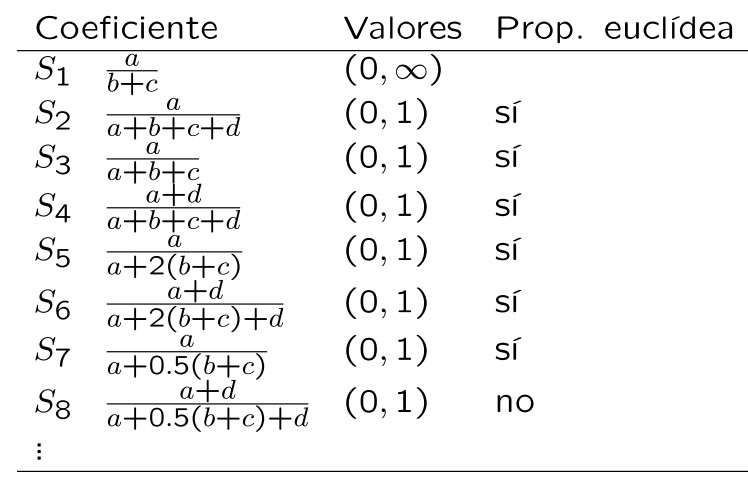
\includegraphics[scale=0.7]{similaridades 1.jpg}

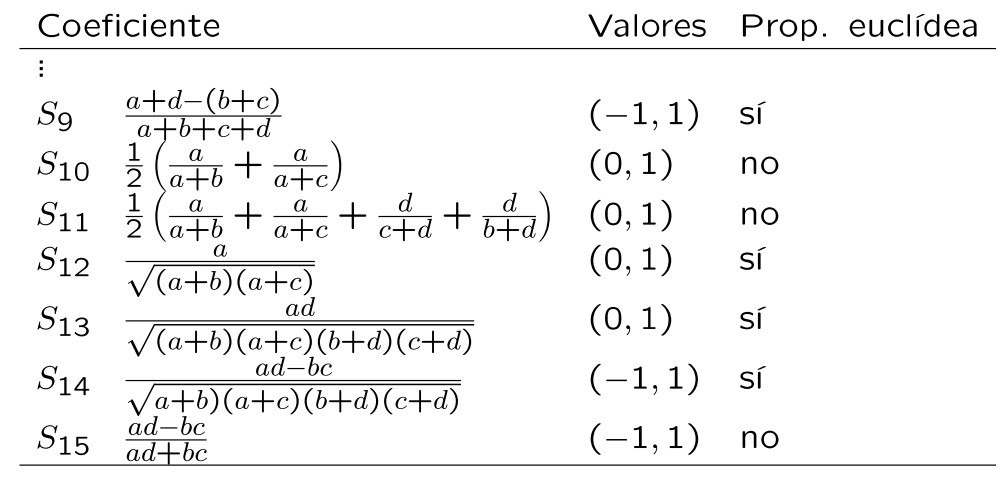
\includegraphics[scale=0.7]{similaridades 2.jpg}

\newpage

\section{Similaridades con variables categoricas múltiples}

Sean $X_1,...,X_p$ variables \textbf{categoricas multiples} (\textbf{no binarias}) con posible distinto numero de categorias.



\tcbset{colback=white!1!white,colframe=brown!78!black}
\begin{tcolorbox}[toptitle=2mm,title=     ]
Los parámetros usados para construir los coeficientes de similaridad con variables categoricas multiples son:

$\alpha_{ij}$ = nº de coincidencias entre las $p$ variables para ambos elementos $i$ y $j$

$p-\alpha_{ij}$ = nº de no coincidencias entre las $p$ variables para ambos elementos $i$ y $j$
\end{tcolorbox}

\subsection{Coeficiente de Coincidencias:}

La medida de similaridad mas habitual en estos casos es el coeficiente de coincidencias:

\tcbset{colback=white!1!white,colframe=brown!78!black}
\begin{tcolorbox}[toptitle=2mm,title=  Coeficiente de Coincidencias:   ]

El coeficiente de coincidencias entre los elementos/individuos $i$ y $j$ respecto de las variables categoricas múlttiples (no binarias) $X_1,...,X_p$ es:

\begin{gather*}
S(i,j)_{Coincidencias}= \dfrac{\alpha_{ij}}{p}
\end{gather*}

\end{tcolorbox}


Observación:

Cuando las variables son binarias el coeficiente de coincidencias coincide con el de Sokal, puesto que $\alpha_{ij}=a_{ij}+b_{ij}$


\subsubsection{Distancia de Coincidencias}

\tcbset{colback=white!1!white,colframe=brown!78!black}
\begin{tcolorbox}[toptitle=2mm,title=  Distancia de Coincidencias:   ]

Obtenemos la distancia de coincidencias:

\begin{gather*}
\delta(i,j)_{Coincidencias} = \sqrt{S(i,i)_{Coincidencias} +S(j,j)_{Coincidencias} - 2\cdot S(i,j)_{Coincidencias} }
\end{gather*}

\end{tcolorbox}

\newpage

\subsection{Aplicación en R:}
\begin{lstlisting}
Datos_Categoricos_Multiples <- Datos_Mixtos%>% select(8:10)
\end{lstlisting}

\includegraphics[scale=1]{datos_multiples.jpg}


\newpage

\subsection{Coeficiente de similaridad de Coincidencias:}

Primero programamos una funcion que nos permita obtener  $\alpha_{i,j}$

\begin{lstlisting}
alpha<- function(i,j, Matriz_Datos_Categoricos_Multiples){
  
  X=as.matrix(Matriz_Datos_Categoricos_Multiples)
  
  alpha=ifelse( X[i,]==X[j,] , yes = 1 , 0)
  
  # Otra forma de hacer lo mismo, pero menos eficiente:
    
  # alpha=rep(0, dim(Matriz_Datos_Categoricos_Multiples)[2])

  # for(k in 1:dim(X)[2]){
  # if( X[i,k]==X[j,k] ){ alpha[k]=1 } else { alpha[k]=0 }
  # }
  
  alpha=sum(alpha)
  
  return(alpha)
}
\end{lstlisting}


\begin{lstlisting}
alpha(1,3 , Datos_Categoricos_Multiples)
\end{lstlisting}

\includegraphics[scale=1]{alpha.jpg}


Ahora programamos el coeficiente de coincidencias:

\begin{lstlisting}
Similaridad_Coincidencias <- function(i,j,   Matriz_Datos_Categoricos_Multiples){

Matriz_Datos_Categoricos_Multiples=as.matrix(Matriz_Datos_Categoricos_Multiples)
  
Similaridad_Coincidencias  =  alpha(i,j, Matriz_Datos_Categoricos_Multiples) / dim(Matriz_Datos_Categoricos_Multiples)[2] 
  
return(Similaridad_Coincidencias )
}
\end{lstlisting}

\newpage

\begin{lstlisting}
Similaridad_Coincidencias(1,3, Datos_Categoricos_Multiples)
\end{lstlisting}

\includegraphics[scale=1]{simCoin1.jpg}

\vspace{0.2cm}

En este caso pasamos de similaridad a distancia usando la transformacion: 
\begin{gather*}
 \delta(i,j)_{Coincidencias}= \sqrt{ S(i,i)_{Coincidencias} + S(j,j)_{Coincidencias} - 2\cdot S(i,j)_{Coincidencias} }
\end{gather*} 
  

\begin{lstlisting}
Dist_Coincidencias <- function(i,j,   Matriz_Datos_Categoricos_Multiples){

Matriz_Datos_Categoricos_Multiples=as.matrix(Matriz_Datos_Categoricos_Multiples)
  
Dist_Coincidencias  = sqrt( Similaridad_Coincidencias(i,i,   Matriz_Datos_Categoricos_Multiples) + Similaridad_Coincidencias(j,j,   Matriz_Datos_Categoricos_Multiples) - 2*Similaridad_Coincidencias(i,j,   Matriz_Datos_Categoricos_Multiples)  )
  
return(Dist_Coincidencias )
}
\end{lstlisting}


\begin{lstlisting}
Dist_Coincidencias(1,3, Datos_Categoricos_Multiples)
\end{lstlisting}


\includegraphics[scale=1]{dist_coin.jpg}

\begin{lstlisting}
Matriz_Similaridad_Coincidencias <- function( Matriz_Datos_Categoricos_Multiples ){
  
  Matriz_Datos_Categoricos_Multiples=as.matrix(Matriz_Datos_Categoricos_Multiples)

  M<-matrix(NA, ncol =dim(Matriz_Datos_Categoricos_Multiples)[1] , nrow=dim(Matriz_Datos_Categoricos_Multiples)[1] )
  
  for(i in 1:dim(Matriz_Datos_Categoricos_Multiples)[1] ){
    for(j in 1:dim(Matriz_Datos_Categoricos_Multiples)[1]){
    
  M[i,j]=Similaridad_Coincidencias(i,j,  Matriz_Datos_Categoricos_Multiples)
  
   }
  }
 return(M)
}
\end{lstlisting}


\begin{lstlisting}
Matriz_Similaridad_Coincidencias(Datos_Categoricos_Multiples) 
\end{lstlisting}


 


\newpage

\subsection{Mas coeficentes de similaridad:}

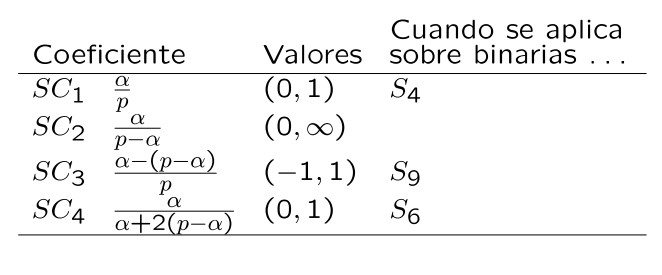
\includegraphics[scale=0.8]{similaridades 3.jpg}






\newpage




\chapter{Distancias con variables de tipo mixto:}

Sean $X=(X_1,...,X_p)$ una matriz de datos de tipo mixto tal que:

$X_1,...,X_{p_1}$ son variables cuantitativas

$X_{p_1 + 1},...,X_{p_1 + p_2}$ son variables categoricas binarias

$X_{p_1 + p_2 + 1},...,X_{p_1 + p_2 + p_3}$ son variables categoricas multiples (no binarias).  

Donde:\hspace{0.2cm} $p=p_1 + p_2 + p_3$

\section{Coeficiente de similaridad de Gower:}

\tcbset{colback=white!1!white,colframe=brown!78!black}
\begin{tcolorbox}[toptitle=2mm,title=  Coeficiente de similaridad de Gower:   ]

El coeficiente de similaridad de Gower entre los elementos $i$ y $j$ respecto de las variables $X_1,...,X_p$ es:

\begin{gather*}
S(i,j)_{Gower}=\dfrac{\sum_{k=1}^{p_1} \left(1- \dfrac{\mid x_{ik} - x_{jk} \mid}{G_k} \right) + a_{ij} + \alpha_{ij} }{p_1 + (p_2 - d_{ij}) + p_3}
\end{gather*}

\end{tcolorbox}

Donde:

$p_1$ es el numero de variables cuantitativas

$p_2$ es el numero de variables categoricas binarias

$p_3$ es el numero de variables categoricas multiples (no binarias)

$G_k$ es el rango de la k-esima variable cuantitativa ( $G_k = max(X_k) - min(X_k)$ )

$a_{ij}$ es el numero de variables binarias (hay $p_2$) para las que las respuesta es 1 en ambos individuos $i$ y $j$

$d_{ij}$ es el numero de variables binarias (hay $p_2$) para las que las respuesta es 0 en ambos individuos $i$ y $j$

$\alpha_{ij}$ es el numero de coincidencias entre las variables categoricas multiples no binarias (hay $p_3$) para los individuos $i$ y $j$


\subsection{Distancia de Gower:}

\tcbset{colback=white!1!white,colframe=brown!78!black}
\begin{tcolorbox}[toptitle=2mm,title=  Distancia de Gower:   ]
La distancia de Gower se obtiene como:

\begin{gather*}
\delta(i,j)_{Gower} = \sqrt{1 - S(i,j)_{Gower}} 
\end{gather*}

\end{tcolorbox}

\newpage
\subsection{Propiedades:}

El coeficiente de similaridad de Gower es la suma de diferentes coeficientes apropiados para cada tipo de variables.

Si solo tenemos variables cuantitativas, la distancia que se obtiene es:

\begin{gather*}
\dfrac{1}{p} \sum_{k=1}^{p } \left(1- \dfrac{\mid x_{ik} - x_{jk} \mid}{G_k} \right)
\end{gather*}

Si solo tenemos variables categoricas binarias, el coeficiente de similaridad de Gower coincide con el de Jaccard.

Si solo tenemos variables categoricas múltiples no binarias,  el coeficiente d Gower coincide con el coeficiente de coincidencias.

\vspace{0.5cm}

Con esta idea pueden construirse otros coeficientes de similaridad para datos de tipo mixto. Algunas recomendaciones para ello son las siguientes:

Si se quiere que el coeficiente resultante tega la propiedad euclidea, todos los coeficientes que se combinen deben tenerla.

Para variables cuantitativas, deben usarse coeficientes que dividan cada comparacion por un factor de normalizacion antes de sumar.

Para variables binarias y cualitativas serán preferibles aquellos coeficientes que tomen valores en [0,1] para evitar rescalar las similaridades antes de sumar

\newpage

\subsection{Aplicación en R: Coeficiente de Gower }

Programamos el coeficiente de Gower:

\begin{lstlisting}
Similaridad_Gower <- function(i,j,   Matriz_Datos_Mixtos, p1, p2, p3){

  X=as.matrix(Matriz_Datos_Mixtos) #tienen que estar las variables ordenadas del siguiente modo: las p1 primeras son cuantitativas, las p2 siguientes son binarias, las p3 siguientes son categoricas multiples (no binarias). De modo que p=p1+p2+p3
  
###################### 
  G<- function(k, X){

  G  =max(X[,k])-min(X[,k])

  return(G)
  }
######################
  
  G_vector<-rep(0, p1)
  
  for(r in 1:p1){
  G_vector[r]=G(r, X)
  }
  
  Matriz_Datos_Binarios = X[ , (p1+1):(p2+p1)]
  
  a= Matriz_Datos_Binarios %*% t(Matriz_Datos_Binarios)
  
  unos<- rep(1, dim(Matriz_Datos_Binarios)[2])

  Matriz_Unos<- matrix( rep(unos, dim(Matriz_Datos_Binarios)[1]),      
                ncol=dim(Matriz_Datos_Binarios)[2])
                
  d= (Matriz_Unos - Matriz_Datos_Binarios)%*%t(Matriz_Unos -     
      Matriz_Datos_Binarios)   
  
  Matriz_Datos_Categoricos_Multiples = X[ , (p1+p2+1):(p1+p2+p3)]
  
  Matriz_Datos_Cuantitativos = X[ , 1:p1]
  
Similaridad_Gower = (  sum( 1 - abs(Matriz_Datos_Cuantitativos[i,] - Matriz_Datos_Cuantitativos[j,])/G_vector ) + a[i,j] + alpha(i,j,Matriz_Datos_Categoricos_Multiples)  ) / (p1+p2- d[i,j] + p3)
  
return(Similaridad_Gower)
}
\end{lstlisting}

\begin{lstlisting}
Similaridad_Gower(1,3, Datos_Mixtos, p1=4, p2=3, p3=3)
\end{lstlisting}

\includegraphics[scale=1]{sim_Gower1.jpg}


\begin{lstlisting}
Matriz_Similaridad_Gower <- function( Matriz_Datos_Mixtos, p1, p2, p3 ){
  
  Matriz_Datos_Mixtos=as.matrix(Matriz_Datos_Mixtos)
  
  M<-matrix(NA, ncol =dim(Matriz_Datos_Mixtos)[1] , nrow=dim(Matriz_Datos_Mixtos)[1] )
  
  for(i in 1:dim(Matriz_Datos_Mixtos)[1] ){
    for(j in 1:dim(Matriz_Datos_Mixtos)[1]){
    
  M[i,j]=Similaridad_Gower(i,j,  Matriz_Datos_Mixtos, p1, p2, p3)
  
   }
  }
 return(M)
}
\end{lstlisting}

\newpage

\begin{lstlisting}
Matriz_Similaridad_Gower(Datos_Mixtos, p1=4, p2=3, p3=3)
\end{lstlisting}

\includegraphics[scale=0.8]{sim_Gower2.jpg}


\vspace{0.4cm}
 
En este caso pasamos de similaridad a distancia usando la transformacion: 
\begin{gather*}
 \delta(i,j)_{Gower}= \sqrt{ 1 - S(i,j)_{Gower} }
\end{gather*} 

 
\begin{lstlisting}
Dist_Gower <- function(i, j, Matriz_Datos_Mixtos , p1, p2, p3) {

Dist_Gower <- sqrt( 1 - Similaridad_Gower(i, j, Matriz_Datos_Mixtos , p1, p2, p3) )

return(Dist_Gower)
}
\end{lstlisting}

 
\begin{lstlisting}
Dist_Gower(1,3, Datos_Mixtos, p1=4, p2=3, p3=3)
\end{lstlisting}

\includegraphics[scale=1]{dist_Gower1.jpg}

\newpage

\begin{lstlisting}
Matriz_Dist_Gower <- function( Matriz_Datos_Mixtos, p1, p2, p3 ){
  
  Matriz_Datos_Mixtos=as.matrix(Matriz_Datos_Mixtos)
  
  M<-matrix(NA, ncol =dim(Matriz_Datos_Mixtos)[1] , nrow=dim(Matriz_Datos_Mixtos)[1] )
  
  for(i in 1:dim(Matriz_Datos_Mixtos)[1] ){
    for(j in 1:dim(Matriz_Datos_Mixtos)[1]){
    
  M[i,j]=Dist_Gower(i,j,  Matriz_Datos_Mixtos, p1, p2, p3)
  
   }
  }
 return(M)
}
\end{lstlisting}

 
 
\begin{lstlisting}
Matriz_Dist_Gower(Datos_Mixtos, p1=4, p2=3, p3=3)
\end{lstlisting}

\includegraphics[scale=0.8]{dist_Gower2.jpg}



\newpage





\section{Coeficiente de similaridad de Gower-Mahalanobis:}

\tcbset{colback=white!1!white,colframe=brown!78!black}
\begin{tcolorbox}[toptitle=2mm,title=  Coeficiente de similaridad de Gower-Mahalanobis:   ]

El coeficiente de similaridad de Gower-Mahalanobis entre los elementos $i$ y $j$ respecto de las variables $X_1,...,X_p$ es:

\begin{gather*}
S(i,j)_{Gower-Maha}=\dfrac{ \left(1- \dfrac{\delta(i,j)_{Maha}}{max(D_{Maha})} \right) + a_{ij} + \alpha_{ij} }{ (p_2 - d_{ij}) + p_3}
\end{gather*}

\end{tcolorbox}

Donde:

$p_2$ es el numero de variables categoricas binarias

$p_3$ es el numero de variables categoricas multiples (no binarias)

$\delta(i,j)_{Maha}$ es la distancia de Mahalanobis entre los individuos respecto de las $p_1$ variables cuantitativas

$max(D_{Maha})$ es el maximo valor de la matriz de distancias de Mahalanobis $\delta(i,j)_{Maha}$ entre los individuos respecto de las $p_1$ variables cuantitativas.

$a_{ij}$ es el numero de variables binarias (hay $p_2$) para las que las respuesta es 1 en ambos individuos $i$ y $j$

$d_{ij}$ es el numero de variables binarias (hay $p_2$) para las que las respuesta es 0 en ambos individuos $i$ y $j$

$\alpha_{ij}$ es el numero de coincidencias entre las variables categoricas multiples no binarias (hay $p_3$) para los individuos $i$ y $j$


\subsection{Distancia de Gower-Mahalanobis:}

\tcbset{colback=white!1!white,colframe=brown!78!black}
\begin{tcolorbox}[toptitle=2mm,title=  Distancia de Gower-Mahalanobis:   ]

La distancia de Gower-Mahalanobis:

\begin{gather*}
\delta(i,j)_{Gower-Maha} = \sqrt{S(i,i)_{Gower-Maha} +S(j,j)_{Gower-Maha} - 2\cdot S(i,j)_{Gower-Maha} }
\end{gather*}

\end{tcolorbox}

\newpage

\subsection{Aplicación en R: Coeficiente de similaridad de Gower-Mahalanobis}

\begin{lstlisting}
Similaridad_Gower_Mahalanobis <- function(i,j,   Matriz_Datos_Mixtos, p1, p2, p3){

  X=as.matrix(Matriz_Datos_Mixtos) 
#tienen que estar las variables ordenadas del siguiente modo: las p1 primeras son cuantitativas, las p2 siguientes son binarias, las p3 siguientes son categoricas multiples (no binarias). De modo que p=p1+p2+p3
  
###################### 
  G<- function(k, X){

  G=max(X[,k])-min(X[,k])

  return(G)
  }
######################
  
  G_vector<-rep(0, p1)
  
  for(r in 1:p1){
  G_vector[r]=G(r, X)
  }
  
  Matriz_Datos_Binarios = X[ , (p1+1):(p2+p1)]
  
  a= Matriz_Datos_Binarios %*% t(Matriz_Datos_Binarios)
  
  unos<- rep(1, dim(Matriz_Datos_Binarios)[2])

  Matriz_Unos<- matrix( rep(unos, dim(Matriz_Datos_Binarios)[1]),      
                ncol=dim(Matriz_Datos_Binarios)[2])
                
  d= (Matriz_Unos - Matriz_Datos_Binarios)%*%t(Matriz_Unos -     
      Matriz_Datos_Binarios)   
  
  Matriz_Datos_Categoricos_Multiples = X[ , (p1+p2+1):(p1+p2+p3)]
  
  Matriz_Datos_Cuantitativos = X[ , 1:p1]
  
  max_maha=max(Matriz_Datos_Cuantitativos)
  
Similaridad_Gower_Mahalanobis = (  1 - Dist_Mahalanobis(i,j,Matriz_Datos_Cuantitativos)/max_maha  + a[i,j] + alpha(i,j,Matriz_Datos_Categoricos_Multiples)  ) / ( p2- d[i,j] + p3 )
  
return(Similaridad_Gower_Mahalanobis)
} 
\end{lstlisting}

 
\vspace{1cm}
 

\begin{lstlisting}
Similaridad_Gower_Mahalanobis(1,2, Datos_Mixtos, p1=4, p2=3, p3=3)
\end{lstlisting}


\begin{lstlisting}
Matriz_Similaridad_Gower_Mahalanobis <- function( Matriz_Datos_Mixtos, p1, p2, p3 ){
  
  Matriz_Datos_Mixtos=as.matrix(Matriz_Datos_Mixtos)
  
  M<-matrix(NA, ncol =dim(Matriz_Datos_Mixtos)[1] , nrow=dim(Matriz_Datos_Mixtos)[1] )
  
  for(i in 1:dim(Matriz_Datos_Mixtos)[1] ){
    for(j in 1:dim(Matriz_Datos_Mixtos)[1]){
    
  M[i,j]=Similaridad_Gower_Mahalanobis(i,j,  Matriz_Datos_Mixtos, p1, p2, p3)
  
   }
  }
 return(M)
}
\end{lstlisting}



\begin{lstlisting}
Matriz_Similaridad_Gower_Mahalanobis(Datos_Mixtos, p1=4, p2=3, p3=3)
\end{lstlisting}




\newpage
 
En este caso pasamos de similaridad a distancia usando la transformacion: 
\begin{gather*}
 \delta(i,j)_{Gower-Maha}= \sqrt{ S(i, i)_{Gower-Maha} + S(j, j)_{Gower-Maha} - 2\cdot S(i,j)_{Gower-Maha} }
\end{gather*} 



\begin{lstlisting}
Dist_Gower_Mahalanobis <- function(i, j, Matriz_Datos_Mixtos , p1, p2, p3) {

Dist_Gower_Mahalanobis <- sqrt( Similaridad_Gower_Mahalanobis(i, i, Matriz_Datos_Mixtos , p1, p2, p3) + Similaridad_Gower_Mahalanobis(j, j, Matriz_Datos_Mixtos , p1, p2, p3) -2*Similaridad_Gower_Mahalanobis(i, j, Matriz_Datos_Mixtos , p1, p2, p3))

return(Dist_Gower_Mahalanobis)
}

\end{lstlisting}

\begin{lstlisting}
Dist_Gower_Mahalanobis(1,2, Datos_Mixtos, p1=4, p2=3, p3=3)
\end{lstlisting}
 
 \vspace{1cm}


\begin{lstlisting}
Matriz_Dist_Gower_Mahalanobis <- function( Matriz_Datos_Mixtos, p1, p2, p3 ){
  
  Matriz_Datos_Mixtos=as.matrix(Matriz_Datos_Mixtos)
  
  M<-matrix(NA, ncol =dim(Matriz_Datos_Mixtos)[1] , nrow=dim(Matriz_Datos_Mixtos)[1] )
  
  for(i in 1:dim(Matriz_Datos_Mixtos)[1] ){
    for(j in 1:dim(Matriz_Datos_Mixtos)[1]){
    
  M[i,j]=Dist_Gower_Mahalanobis(i,j,  Matriz_Datos_Mixtos, p1, p2, p3)
  
   }
  }
 return(M)
}
\end{lstlisting}


\begin{lstlisting}
Matriz_Dist_Gower_Mahalanobis(Datos_Mixtos, p1=4, p2=3, p3=3)
\end{lstlisting}
 


 







\end{document}
